\chapter{Time Series Methods for Air Quality}

With the proliferation of low-cost sensors for a wide range of IoT and wearable biometric applications, a systematic approach to both quality control and performing comprehensive time series analysis has significant value. It is highly desirable to be able to answer some basic questions using \textit{just} the time series alone. For example: What is the likely sensor uncertainty given a time series of observations? How frequently should observations be made to adequately resolve typical temporal variability? How representative is a single observation of what one expects to see over a temporal (and spatial) window? Can we construct predictive models for the time series of a single sensor given a sufficient volume of sample data? In this chapter we seek to address these questions with direct application to the data collected by our low cost air quality sensor network. First, we will demonstrate how the \textit{temporal variogram} provides a way to assess the intrinsic sensor uncertainty from a time series, and in the process, develop an open-source Julia implementation of a variety of variogram methods that can be used for any generic time series. Next, we present two techniques for physics-based time series modeling: the Hankel Alternative View Of Koopman (HAVOK) method, and the Hamiltonian Neural Network. It should be noted that despite the rapid pace of development in the fields of data-driven and scientific machine learning, many recently developed techniques like the Universal Differential Equations (UDEs), Hamiltonian Neural Networks, and others have yet to see wide spread application on noisy, real-world datasets. Our secondary goal for this chapter is therefore to demonstrate how, with some slight modifications, these techniques can be applied to real-world problems.



\section{Time-Series Methods for Uncertainty Quantification}

As we've already demonstrated, the shrinking cost of sensing technologies has improved our ability to create dense sensing networks. In order to make effective use of these sensors, and to provide high quality data that can be used for critical decision making, it is vital we establish both the relevant sampling time scale and reasonable uncertainty estimates for measurements obtained by these sensors. For low cost sensors in particular, the manufacture supplied uncertainty estimates tend to be highly conservative so as to minimize their responsibility for variation in device performance, and in general, to prevent unnecessary returns. Consider for example, the sample time series for particulate matter concentrations at a variety of size fractions collected by one of our low-cost sensing nodes for a single 24-hour period (figure \ref{fig:pm-single-day}:
\begin{figure}[h]
  \centering
  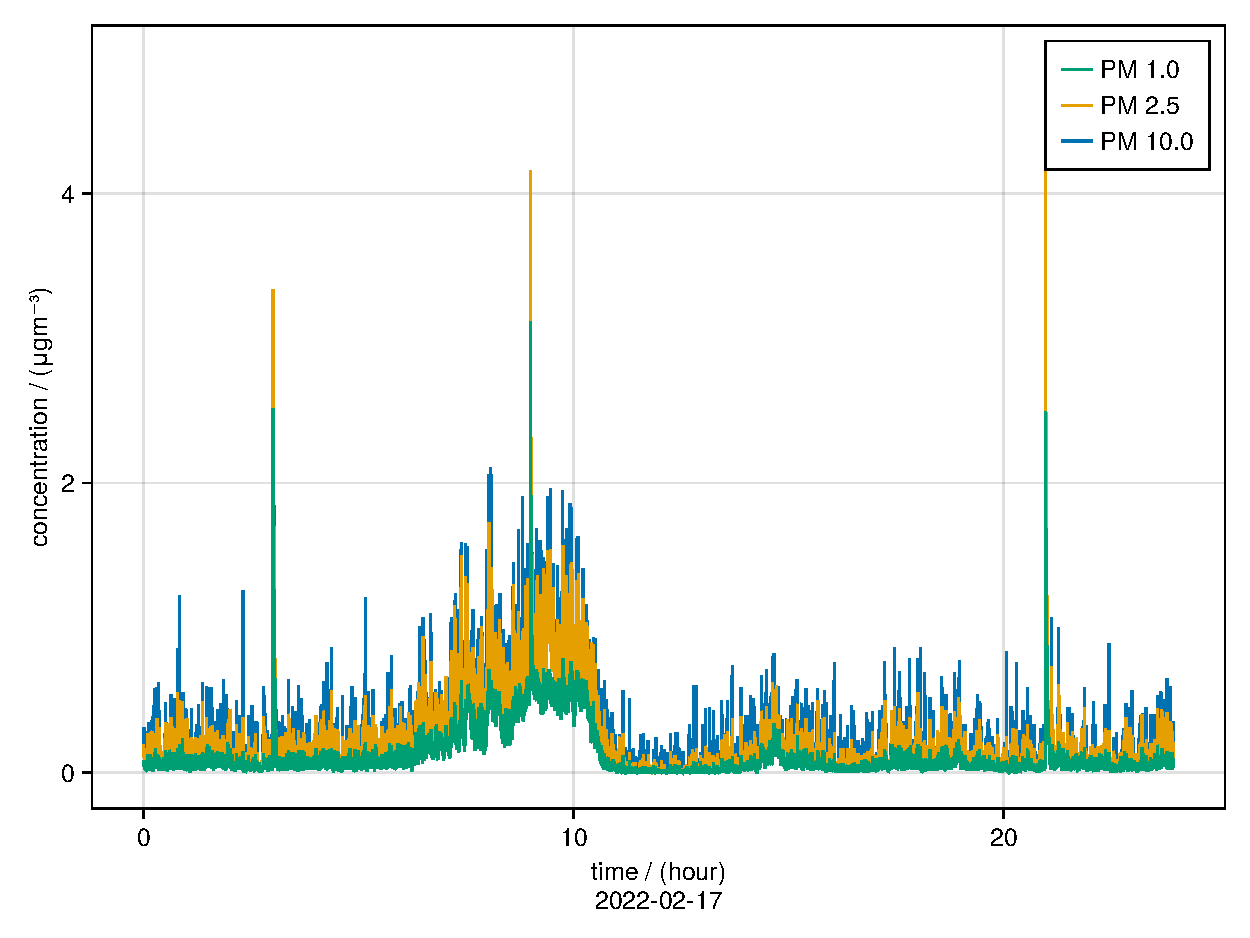
\includegraphics[width=0.85\columnwidth]{time-series/variogram/single-day/IPS_single-day.pdf}
  \caption{Time series of particulate matter at size fractions $1.0$, $2.5$, and $10.0$ $\mu m$ captured at a single location over one 24-hour day.}
  \label{fig:pm-single-day}
\end{figure}
These sample data illustrate many typical features of air quality time series: there is a baseline level of noise, there are general periodic trends (an increase in concentration at all size fractions near morning traffic around hour 10), and there are intermittent transient events. If we suppose that we \textit{already} know what the shortest time resolution needed to resolve the important transients is, say $\Delta t$, then a straight forward approach to develop a baseline notion of uncertainty for a time series, $z(t)$, is to convolve a rolling window of width $\Delta t$ across the signal so that at any time $t$ we may define the associated \textit{pseudo-observation} to be
\begin{equation}
  \bar{z}(t) = \text{mean}\left(\left\{z_j \right\}\right) \pm \text{std}\left(\left\{z_j \right\}\right); \quad \text{where } j \in \left\{ \left. j \right\vert t - \frac{\Delta t}{2} \leq t_j  \leq t + \frac{\Delta t}{2}\right\}
\end{equation}
where $\text{std}\left(\left\{z_j\right\}\right)$ is called the \textit{representativeness uncertainty} as it measures how representative a single measurement is for the entire sampling window.

Unfortunately it may be difficult to know the relevant times scales of key transient events in advance. Given the fact that it is increasingly common for modern sensing systems (like our low-cost PM monitors) to provide sampling rates north of 1 Hz, we do not want to \textit{shoot ourselves in the foot} by arbitrarily choosing an averaging window that will smooth away all the relevant features. Therefore, we seek to develop an alternative technique that can simultaneously establish the relevant temporal resolution for sampling whilst also enabling us to estimate the aleatoric, that is, intrinsic uncertainty of the sensing system.

\subsection{Uncertainty Quantification with Temporal Variograms}

The key feature that differentiates time series from other data sources is that at short time scales, neighboring samples are not independent; measurements taken close in time tend to be more correlated than measurements taken far apart. One way to measure this idea of self-similarity is by the auto-correlation function, which for a continuous signal $z(t)$ is
\begin{equation}
  R_{zz}(\Delta t) = \int_\infty^\infty z(t +\Delta t)z^*(\Delta t)dt.
\end{equation}
This can be efficiently computed for real-valued time series in $\mathcal{O}(n\log n)$ using the \textit{Fast Fourier Transform} via
\begin{equation}
  R_{zz}(\Delta t) = \mathcal{F}^{-1}\left[\mathcal{F}(z)\cdot (\mathcal{F}(z))^*\right]
\end{equation}
The first peak of this autocorrelation function is an excellent method to identify the relevant time-scale: high autocorrelation means we gain little extra information between points offset by a time lag of $\Delta t$. This puts us on the right track but does not provide a straight forward interpretation for an intrinsic uncertainty. Taking motivation from the representativeness uncertainty, let us instead consider the expected variance between neighboring samples as a function of the time lag $\Delta t$. That is,
\begin{equation}
  2\gamma(\Delta t) =  \text{Var}\left(z(t+\Delta t) - z(t)\right)
\end{equation}
where $\gamma$ is called the \textit{semi-variogram} for $z(t)$. Expanding this definition yields
\begin{equation}
  2\gamma(\Delta t) = \E\left[\left(z(t+\delta t) - z(t) - \E\left(z(t+\Delta t) - z(t) \right) \right)^2 \right]
\end{equation}
which for timescales where $z(t)$ is sufficiently stationary simplifies to yield
\begin{equation}
  \gamma(\Delta t) = \frac{1}{2}\E\left[ \left(z(t+\Delta t) - z(t) \right)^2\right].
\end{equation}

For a perfect measurement system we would expect that taking $\lim_{\Delta t \to 0}\gamma(\Delta t) = 0$, since measurements taken at the same time by the same instrument \textit{should} be identical. Intrinsic uncertainty will therefore manifest as a non-zero limit and taking the square-root of the variogram will yield units that match our original time series and provide a reasonable uncertainty estimate. For a given set of samples, we construct the \textit{empircal variogram} as
\begin{equation}
  \hat{\gamma}(\Delta t) = \frac{1}{2N(\Delta t)}\sum_i^{N(\Delta t)}\left(z(t_i + \Delta t) - z(t_i) \right)^2
\end{equation}
where $N(\Delta t)$ are the number of available observation pairs $(z_i, z(t_i+\Delta t))$ for a lag of $\Delta t$.

There are three key parameters of the variogram $\gamma(\Delta t)$ which we want to estimate from $\hat{\gamma}(\Delta t)$:
\begin{itemize}
\item \textbf{Nugget}: The $y$-intercept of $\gamma(\Delta t)$ representing the limit as $\Delta t \to 0$.
\item \textbf{Sill}: The value of $\gamma(\Delta t)$ as $\Delta t \to \infty$. In other words, the expected variance for uncorrelated samples of our time series. \textit{Note} the \textbf{partial sill} is defined to be the sill minus the nugget.
\item \textbf{Range}: The $\Delta t$ at which $\gamma$ realizes it asymptote. Effectively this is the time lag beyond which samples are uncorrelated and can be used as a proxy for the relevant sampling time scale.
\end{itemize}

To do this, we first compute $\hat{\gamma}(\Delta t)$ as above and then fit a model to $\gamma(\Delta t)$. There are a number of popular choices depending on the structure of a particular time series. In my open source Julia implementation, \texttt{TimeSeriesTools.jl}, the following models are made available:
\begin{itemize}
\item \textbf{Spherical}:
  \begin{equation}
    \gamma(\Delta t) = b + C_0\left(1.5\frac{\Delta t}{r} - 0.5 \frac{(\Delta t)^2}{r^2} \right)
  \end{equation}
\item \textbf{Exponential}:
  \begin{equation}
    \gamma(\Delta t) = b + C_0\left( 1 - \exp\left(-\frac{\Delta t}{r}\right)\right)
  \end{equation}
\item \textbf{Gaussian}:
  \begin{equation}
    \gamma(\Delta t) = b + C_0\left( 1 - \exp\left(-\frac{(\Delta t)^2}{r^2}\right)\right)
  \end{equation}
\item \textbf{Circular}:
  \begin{equation}
    \gamma(\Delta t) = b + C_0\left(1 - (2\pi)\cos^{-1}\left(\frac{\Delta t}{r}\right) + \frac{2\Delta t}{\pi r}\sqrt{1-\frac{(\Delta t)^2}{r^2}} \right)
  \end{equation}
\item \textbf{Cubic}:
  \begin{equation}
    \gamma(\Delta t) = b + C_0\left(7\left(\frac{\Delta t}{r} \right)^2 - 8.75 \left(\frac{\Delta t}{r} \right)^3 + 3.5\left(\frac{\Delta t}{r} \right)^5 - 0.75\left(\frac{\Delta t}{r} \right)^7 \right)
  \end{equation}
\item \textbf{Pentaspherical}:
  \begin{equation}
    \gamma(\Delta t) = b + C_0 \left( \frac{15}{8}\left(\frac{\Delta t}{r} \right) - \frac{5}{4}\left(\frac{\Delta t}{r} \right)^3 + \frac{3}{8}\left(\frac{\Delta t}{r}\right)^5 \right)
  \end{equation}
\item \textbf{Sine Hole}
  \begin{equation}
    \gamma(\Delta t) = b + C_0\left(1 - \frac{\sin(\pi\Delta t/r)}{\pi\Delta t/r}\right)
  \end{equation}
\end{itemize}
where $C_0$ is the partial sill, $b$ is the nugget, and $r$ is the range. Figure \ref{fig:pm10-variogram-fits} demonstrates these fits for the $\text{PM}_{10}$ time series from above.

\begin{figure}[h]
  \centering
  \includegraphics[width=0.85\columnwidth]{time-series/variogram/single-day/γ-PM 10.0_single-day.pdf}
  \caption{The empirical variogram and a variety of model fits obtained for the a PM $10.0$ single-day time series}
  \label{fig:pm10-variogram-fits}
\end{figure}

\subsection{Next Steps}

As of right now, I have developed an open source library to compute the temporal variogram and extract the estimated uncertainty for generic time series data. I have also developed a pipeline for the acquisition and storage of time series data in publicly available S3 buckets on the Open Storage Network. My plan now is to evaluate the uncertainty for a variety of sensors from our network for data collected across the previous 1-3 years. We will then be able to investigate how stable these uncertainty estimates are as a function of time. For example, do we see any seasonal trends during the coldest winter months and warmest summer months? Does the uncertainty appear to increase over time so that we might be able to automatically identify when a sensor should be serviced/replaced? 



\section{Physics Informed modeling techniques for Air Quality Data}


In order to provide actionable insights we must be able to effectively model the dynamics of our collected time series. In a perfect world, we would measure all relevant physical quantities such that the time evolution of local air quality at each sensor could be obtained by simulating the relevant micro-physics. However, low cost sensor networks are not equipped with all the necessary reference grade instruments needed to perform such simulations; accurate winds speed and direction sensors alone can cost hundreds to thousands of dollars and remote sensing data products are often unreliable at the ground level (i.e. in the human head space). We therefore are motivated to develop techniques to model our collected time series using only the data provided at a single node. There are many approaches to this task in the statistics and machine learning literature including statistical models like ARIMA and deep learning methods like Recurrent Neural Networks \cite{intro-to-time-series-models, time-series-rnns}. While these methods can often lead to robust short term predictions, they do not incorporate prior physics knowledge and therefore are not primed to take advantage of underlying dynamical laws. Recently two interesting physics-informed, data driven techniques have been developed for just this type of scenario. The first we shall examine is the so-called \textit{Hankel Alternative View Of Koopman} (HAVOK) framework which extends the principle of dynamic mode decomposition to nonlinear systems \cite{brunton-havok}. The second is an technique dubbed the \textit{Hamiltonian Neural Network} which extends the notion of a Neural Ordinary Differential Equation to allow a neural network to learn coordinate transformations or the original time series data which satisfy \textit{Hamiltons equations} \cite{greydanus-hnn}.

\subsection{A Hybrid HAVOK UDE Approach}

If we are to take a physics informed approach to modeling our time series, a good place to start is with the question: \textit{How much information about the physical state of a system can be extracted from a single time series}. The answer, surprisingly, is \textit{more than you might expect}. For simplicity let us consider a discrete, deterministic dynamical system described by a smooth function $f:M\to M$ that maps points in the state-space manifold $M$ to new points in the same manifold. We can define an \textit{observable} $y:M\to\R$ as a smooth function which maps a state $x_t\in M$ to a number. The Takens Embedding Theorem then suggests that if the dynamical system described by $f$ has a strange attractor of box counting dimension $d$, then there exists a $k\geq 2d$ such that the embedding $\mathbf{y}:M\to\R^k$ given by
\begin{equation}
  \mathbf{y}(x) = \left(y(x), y(f(x)), y(f^2(x)), ..., y(f^{k-1}(x)) \right)
\end{equation}
is a diffeomorphism. In other words, the time series $(y(x_t), y(x_{t+1}), y(x_{t+2}),...)$ formed by tracking the evolution of a single point $x_t$ in the state manifold $M$ under the dynamical law $x_k\mapsto x_{k+1}=f(x_k)$ captures the entire structure of the original dynamics in the state manifold \cite{takens-theorem}. This remarkable result provides justification for our modeling and suggests that for practical purposes, we will want to construct our models by considering dynamics on vectors formed by so called \textit{time delay embeddings} like that of the previous equation.

With this justification in hand, the next logical step is to propose a model for the dynamics which describe the evolution of such delay-embeddings. To do this, we will utilize technqieus from Koopman Operator theory. Koopman operator theory provides a framework for understanding the time evolution of a dynamical system at the level of observable functions rather than directly from the state itself. This is highly analogous to the equivalence between the Schrodinger and Heisenberg pictures in Quantum Mechanics where the former provides time evolution via dynamics of the state vector, $\vert \alpha(t) \rangle$, and the later provides dynamics on the observable operators, $X(t)$, of a system \cite[p 80-84]{sakurai-qm}. In this same spirit, we seek to identify an operator $\mathcal{K}$, called the \textit{Koopman Operator} for our dynamical system which satisfies
\begin{equation}
  \mathcal{K}\left[y(x_k) \right] = y(f(x_k)) = y(x_{k+1}),
\end{equation}
that is, $\mathcal{K}$ takes an observable $y$ and maps it to a new value which is just the observable evaluated at the \textit{next} state after an update from $f$. This is highly appealing because such an operator (if it exists) is \textit{linear} and results in a \textit{linear} dynamical system for the time series of an observable, namely
\begin{equation}
  y_t = \mathcal{K}^t(y_0) = y(f^t(x_0)).
\end{equation}

The goal should now be clear: if we are able to utilize the data from our time series (interpreted as an \textit{observable} of the underlying system's state space) to estimate the operator $\mathcal{K}$, then we will be able to model the dynamics of our time series for which a time delay embedding of sufficient length should produce an attractor that is diffeomorphic to the underlying dynamics of the system's true state. Unfortunately, the price paid for the linearity of $\mathcal{K}$ is that its representation may demand an infinite dimensional basis \cite{brunton-modern-koopman}. Therefore, in practice, we hope that sufficient data will enable us to identify a suitable subspace of $M$ for which a finite approximation of $\mathcal{K}$, say $K$, keeps our observables bounded. One approach \textcolor{red}{(add citation for Mezic et al here)} is to attempt an eigen decomposition of $K$ using our time series data which relies on carefully crafting the observable functions $y$. In our case, we do not have direct control over the available observables; we are limited to the sensors provided by each sensing node. As an alternative approach, we take inspiration from the popular method of Dynamic Mode Decomposition (DMD) to enable approximations of the Koopman operator from time series observations.

Originally, DMD was introduced to allow for the decomposition of expensive fluid dynamics simulations into a basis of \textit{modes} (in the spirit of normal modes) such that the time evolution across the entire domain can be obtained by a linear combination of such modes with some simple time-dependent coefficients. With this as our inspiration, we can take a similar approach by forming a so called \textit{Hankel matrix}, $H$, from our time series as
\begin{equation}
  H = \begin{bmatrix}
    y_1 & y_2 & ... & y_p \\
    y_2 & y_3 & ... & y_{p+1} \\
    \vdots & \vdots & \ddots & \vdots \\
    y_q & y_{q+1} & ... & y_{p+q}
    \end{bmatrix}
\end{equation}
\textcolor{red}{(NOTE: we should update this to match our definition i.e. starting at $y_1$ or $y_q$ as the first element)} where each column is a shifted time delay embedding of length $q$ and each row corresponds to a subsample of our observable time series of length $p$. We can decompose this matrix using the SVD so that
\begin{equation}
  H = U\Sigma V^T,
\end{equation}
where the singular values $\sigma_k=\Sigma_{kk}$ are ranked hierarchically by the relative contribution to $H$. If the singular values drop off fast enough, a reasonable approximation to $H$ can be obtained by keeping only $r$-many singular values and singular vectors from the decomposition. This provides us a data-driven approach to approximating the Koopman operator for a subspace (that is a subset of singular vectors) that is approximately invariant. To see this, we can rewrite our Hankel matrix in terms of $\mathcal{K}$ so that
\begin{equation}
  H = \begin{bmatrix}
    y_1 & \mathcal{K}(y_1) & ... & \mathcal{K}^{p-1}(y_1) \\
    \mathcal{K}(y_1) & \mathcal{K}^2(y_1) & ... & \mathcal{K}^p(y_1) \\
    \vdots & \vdots & \ddots & \vdots \\
    \mathcal{K}^{q-1}(x_1) & \mathcal{K}^q(x_1) & ... & \mathcal{K}^{p+q-1}(x_1)
    \end{bmatrix}
\end{equation}
this direct connection to the propagation by $\mathcal{K}$ suggests we \textit{should} be able to successfully obtain a linear model describing the dynamics of the singular vectors $v_i(t)$. The potential for multiple attractors as well as the challenges of noise in real datasets suggests that a linear model alone may not be good enough to recover the full dynamics and therefore the HAVOK model proposed by Brunton seeks to fit a model on the first $r-1$ singular vectors with \textit{external forcing} provided by the r\textsuperscript{th} component:
\begin{equation}
  \frac{d}{dt}\mathbf{v}(t) = A\mathbf{v}(t) + Bv_r(t)
\end{equation}
where $\mathbf{v} = \left(v_1, v_2, ..., v_{r-1}\right)^T$. To demonstrate this approach, consider the famous Lorenz dynamical system given by
\begin{align}
  \dot{x} = \sigma(y-x) \\
  \dot{y} = x(\rho-z) -y \\
  \dot{z} = xy - \beta z
\end{align}
with parameters chosen so that $\sigma = 10$, $\rho=20$, and $\beta=8/3$. Because the SVD provides a hierarchical ranking of the singular vectors by the relative scale of the singular values, we imagine this $v_r(t)$ to be an intermitent external forcing do the the fact that it represents a low energy mode. A visualizualition of a sample trajectory for this system as well as the \textit{embedded} attractor formed from the first three principal vectors $v_1, v_2, v_3$ of the singular value decomposition of the associated Hankel matrix for the ``observable'' $x(t)$ are illustrated in Figure \ref{fig:lorenz-attractor}.
\begin{figure}[h]
  \centering
  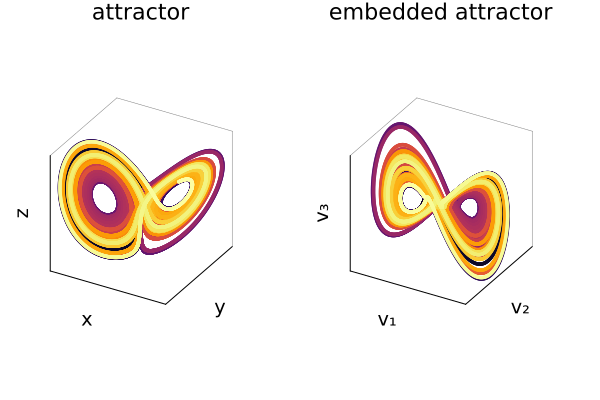
\includegraphics[width=0.85\columnwidth]{time-series/HAVOK/lorenz/havok/attractors1.png}
  \caption{Comparing the original Lorenz attractor (left) to the embedded attractor learned after performing the SVD (right). Color indicates the time along the trajectory.}
  \label{fig:lorenz-attractor}
\end{figure}

This is a clear demonstration of Takens embedding theorem in action: the attractor formed from the first three singular vectors of the Hankel matrix for the single observable $x(t)$ appear to capture key features of the original attractor formed from the state vector $(x(t), y(t), z(t))^T$. The rows of the matrix $U$ correspond to the \textit{modes} of the singular value decomposition and allow us to decompose the original delay embedding of the observable time series into this new representation. In this example, we have chosen $r=15$ as is done in \cite{brunton-havok}. A more programmatic approach is to evaluate $r$ based on some information criterion. Alternatively, this can be left as a hyperparameter and adjusted to achieve a better fit. These modes are visualized in Figure \ref{fig:lorenz-modes} below.

\begin{figure}[h!]
  \centering
  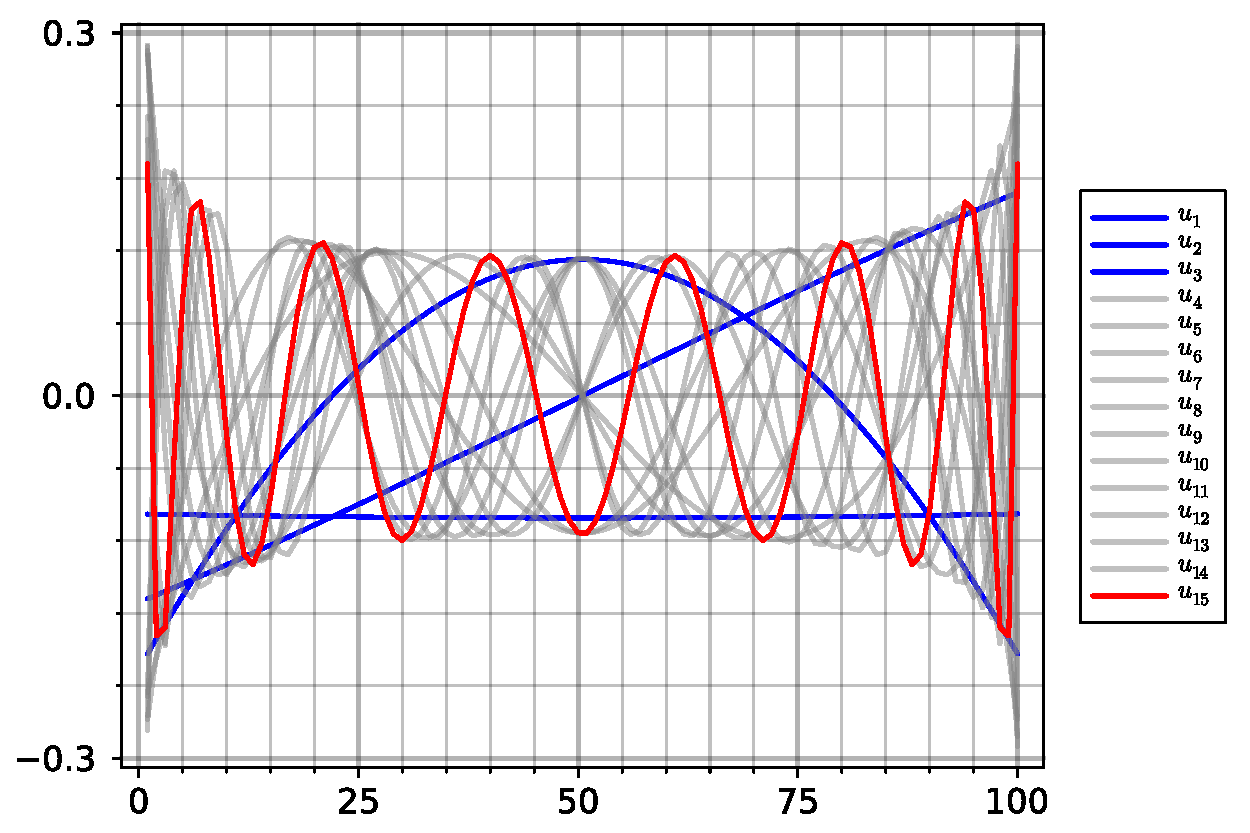
\includegraphics[width=0.85\columnwidth]{time-series/HAVOK/lorenz/havok/eigenmodes.pdf}
  \caption{Eigenmodes of the embedded attractor extracted from the SVD.}
  \label{fig:lorenz-modes}
\end{figure}

The matrices $A$ and $B$ for our HAVOK model are obtained by standard linear regression. \textcolor{red}{(We should add further description of how to form the linear system here, .e.g. we do linear regression on a non-square matrix of weights to let us fit A and B simultaneously.)} The coefficients of these matrices for the Lorenz system described above are illustrated in Figure \ref{fig:lorenz-coeffs}. We note that the form of the $A$ matrix appears to closely follow the Toeplitz structure one would expect from the matrix of a finite difference stencil.
\begin{figure}[h!]
  \centering
  \includegraphics[width=0.85\columnwidth]{time-series/HAVOK/lorenz/havok/heatmap.pdf}
  \caption{Heatmap of the linear Koopman operator together with the forcing activation.}
  \label{fig:lorenz-coeffs}
\end{figure}
We can then examine the time series obtained by integrating the HAVOK model forward to see how well we model the original dynamics of the singular vectors $v_i$. The first of these is shown in Figure \ref{fig:lorenz-v1}
\begin{figure}[h!]
  \centering
  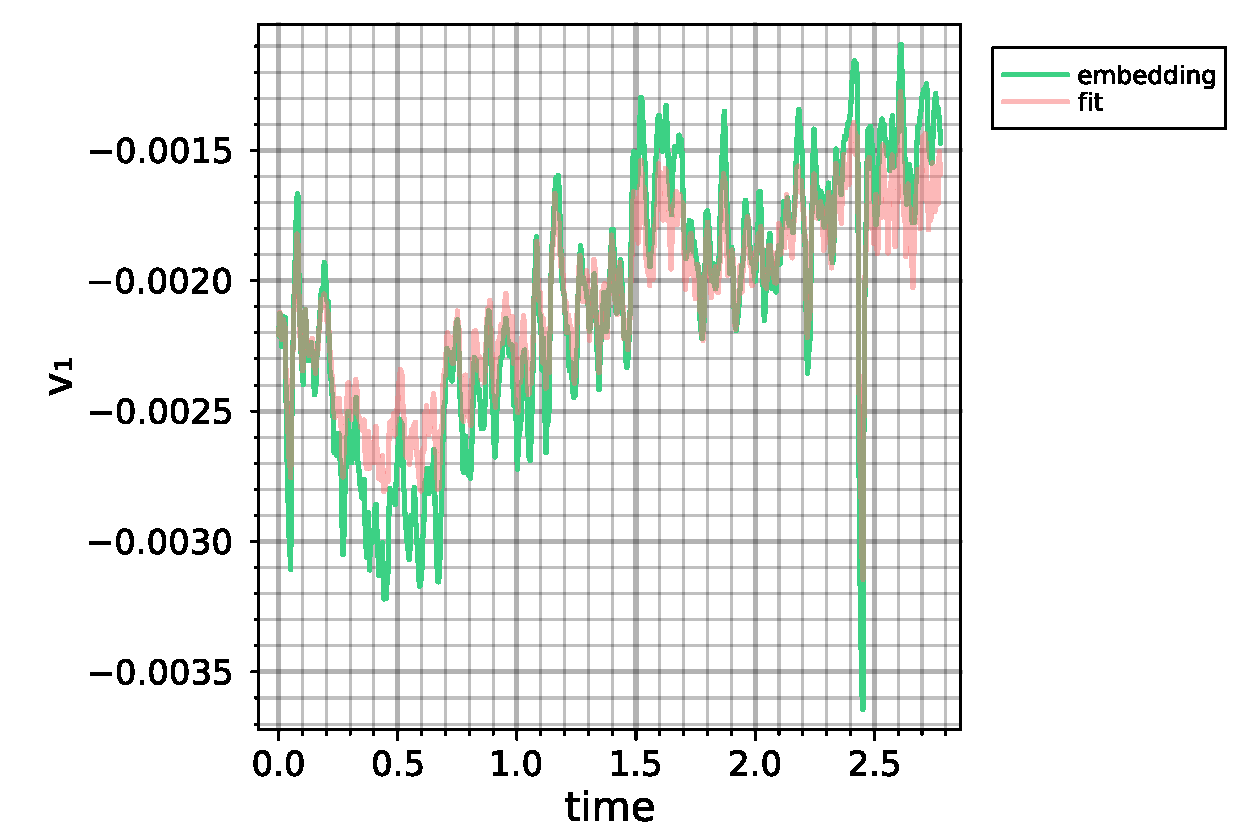
\includegraphics[width=0.85\columnwidth]{time-series/HAVOK/lorenz/havok/timeseries_reconstructed.pdf}
  \caption{The reconstructed timeseries for $v_1$ via the learned HAVOK model.}
  \label{fig:lorenz-v1}
\end{figure}
To further evaluate the quality of the resulting model, we can visualize the scatter diagram of the predicted values for $v_1(t)$ on training data (the points that were used in the Hankel Matrix) as well as some holdout data. The results are shown in Figure \ref{fig:lorenz-scatter}.
\begin{figure}[h!]
  \centering
  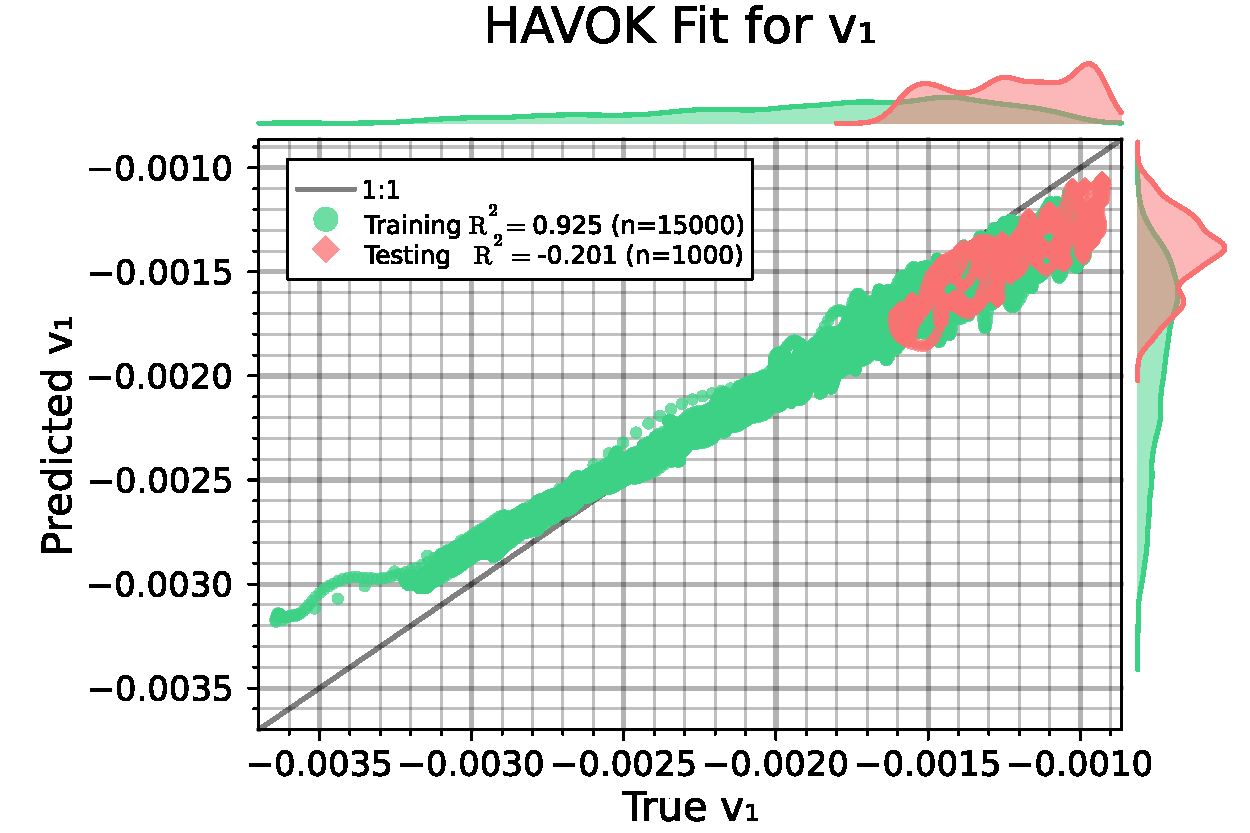
\includegraphics[width=0.85\columnwidth]{time-series/HAVOK/lorenz/havok/scatterplot.pdf}
  \caption{A scatterplot of the resulting HAVOK fit}
  \label{fig:lorenz-scatter}
\end{figure}

\begin{figure}[!hbt]
  \centering
  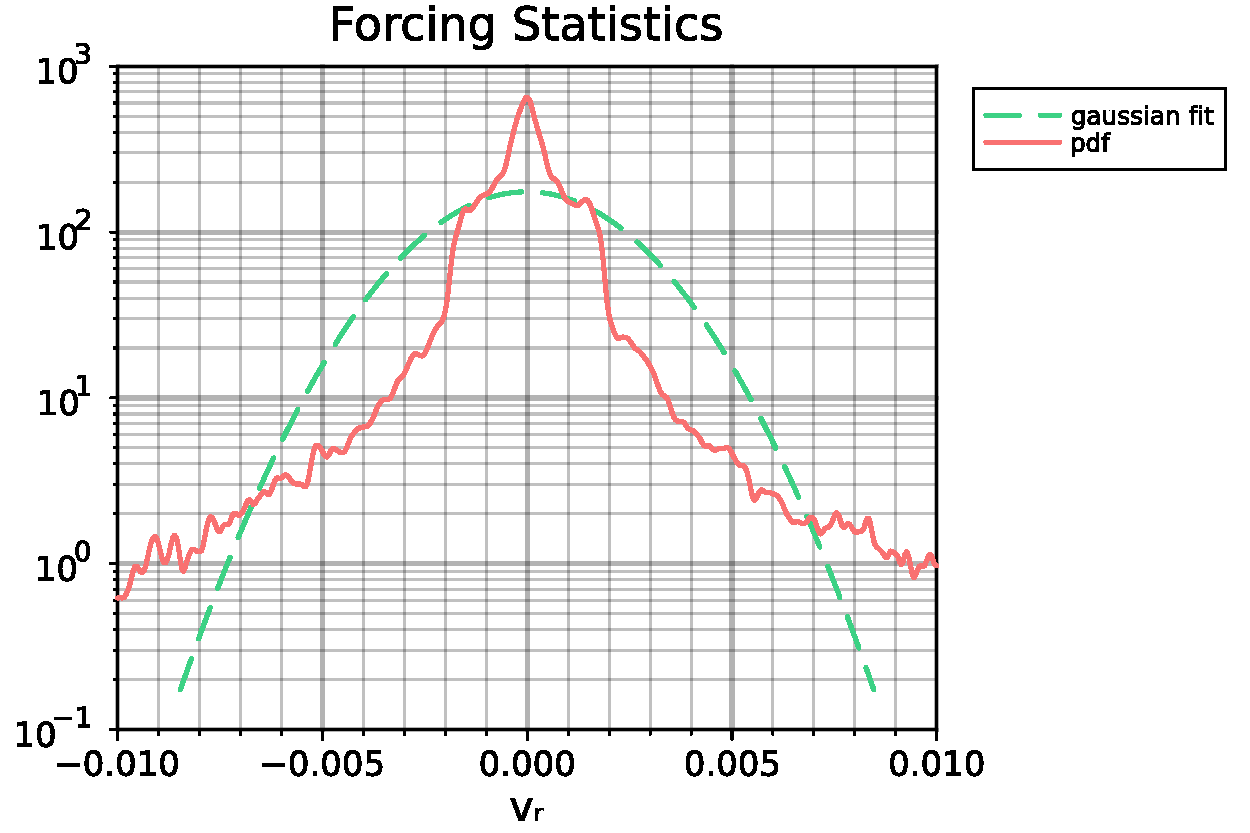
\includegraphics[width=0.85\columnwidth]{time-series/HAVOK/lorenz/havok/forcing-stats.pdf}
  \caption{The statistics of the learned forcing function. The sharpness of the distribution (in comparison to a Normal distribution) indicates that the forcing is \textit{intermittent}}
\end{figure}


Finally, we can visualize the original time series series and the embedded attractor by differentiating regions with high externel forcing (salmon colored) from the regions where the observable is approximately linear (green colored), that is where the dynamics of the observable are invariant to our learned Koopman operator. This is illustrated in Figures \ref{fig:lorenz-forcing} and \ref{fig:lorenz-attractor-forcing}.
\begin{figure}[!hbt]
  \centering
  \includegraphics[width=0.85\columnwidth]{time-series/HAVOK/lorenz/havok/v1_forcing_identified.pdf}
  \caption{The time series for $v_1$ marked where the forcing function is above a specified threshold.}
  \label{fig:lorenz-forcing}
\end{figure}

\begin{figure}[!hbt]
  \centering
  \includegraphics[width=0.85\columnwidth]{time-series/HAVOK/lorenz/havok/attractor_w_forcing.png}
  \caption{The embedded attractor colored by the presence of external forcing.}
  \label{fig:lorenz-attractor-forcing}
\end{figure}


\subsubsection{Results so far}

What happens if we try and apply this HAVOK approach to a sample of our PM time series? This section details preliminary results with the method. Figure \ref{fig:attractor-pm} illustrated the embedded attractor obtained by visualizing the first 3 singular vectors of the SVD for a $\text{PM}_{2.5}$ time series.
\begin{figure}[!hbt]
  \centering
  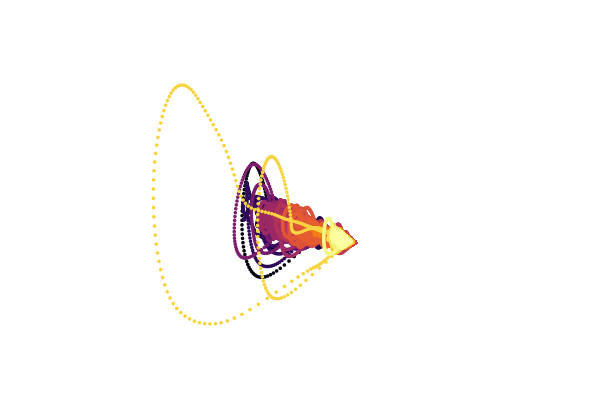
\includegraphics[width=0.85\columnwidth]{time-series/HAVOK/sharedair/havok/attractor.png}
  \caption{The embedded attractor for PM $2.5$ time-series data.}
  \label{fig:attractor-pm}
\end{figure}
After attempting a variety of cut of values $r$ as well as a variable number of forcing terms, the \textit{best fit} values for the $A$ and $B$ matrices are visualized in \ref{fig:pm-a-b-mats}. As in the case of the Lorenz system, the $A$ matrix has an interesting structure of alternating positive and negative coefficients in an anti-symmetric pattern along the diagonals. The learned coefficients of the external forcing activation matrix $B$ appear to be biased towards negative values.
\begin{figure}[h]
  \centering
  \includegraphics[width=0.85\columnwidth]{time-series/HAVOK/sharedair/havok/heatmap.pdf}
  \caption{Heatmap of the linear Koopman operator together with the forcing activation.}
  \label{fig:pm-a-b-mats}
\end{figure}
Time series obtained for the first three components are visualized in Figure \ref{fig:pm-timeseris-long}. In figure \ref{fig:pm-timeseries-zoomed} we show the same data limited to the first 2.5 hours. This appears to suggest that the HAVOK models has learned a reasonable representation of the dynamics, however errors appear to accumulate over past 2.5 hours such that the model fails for long time integration.
\begin{figure}[h]
  \centering
  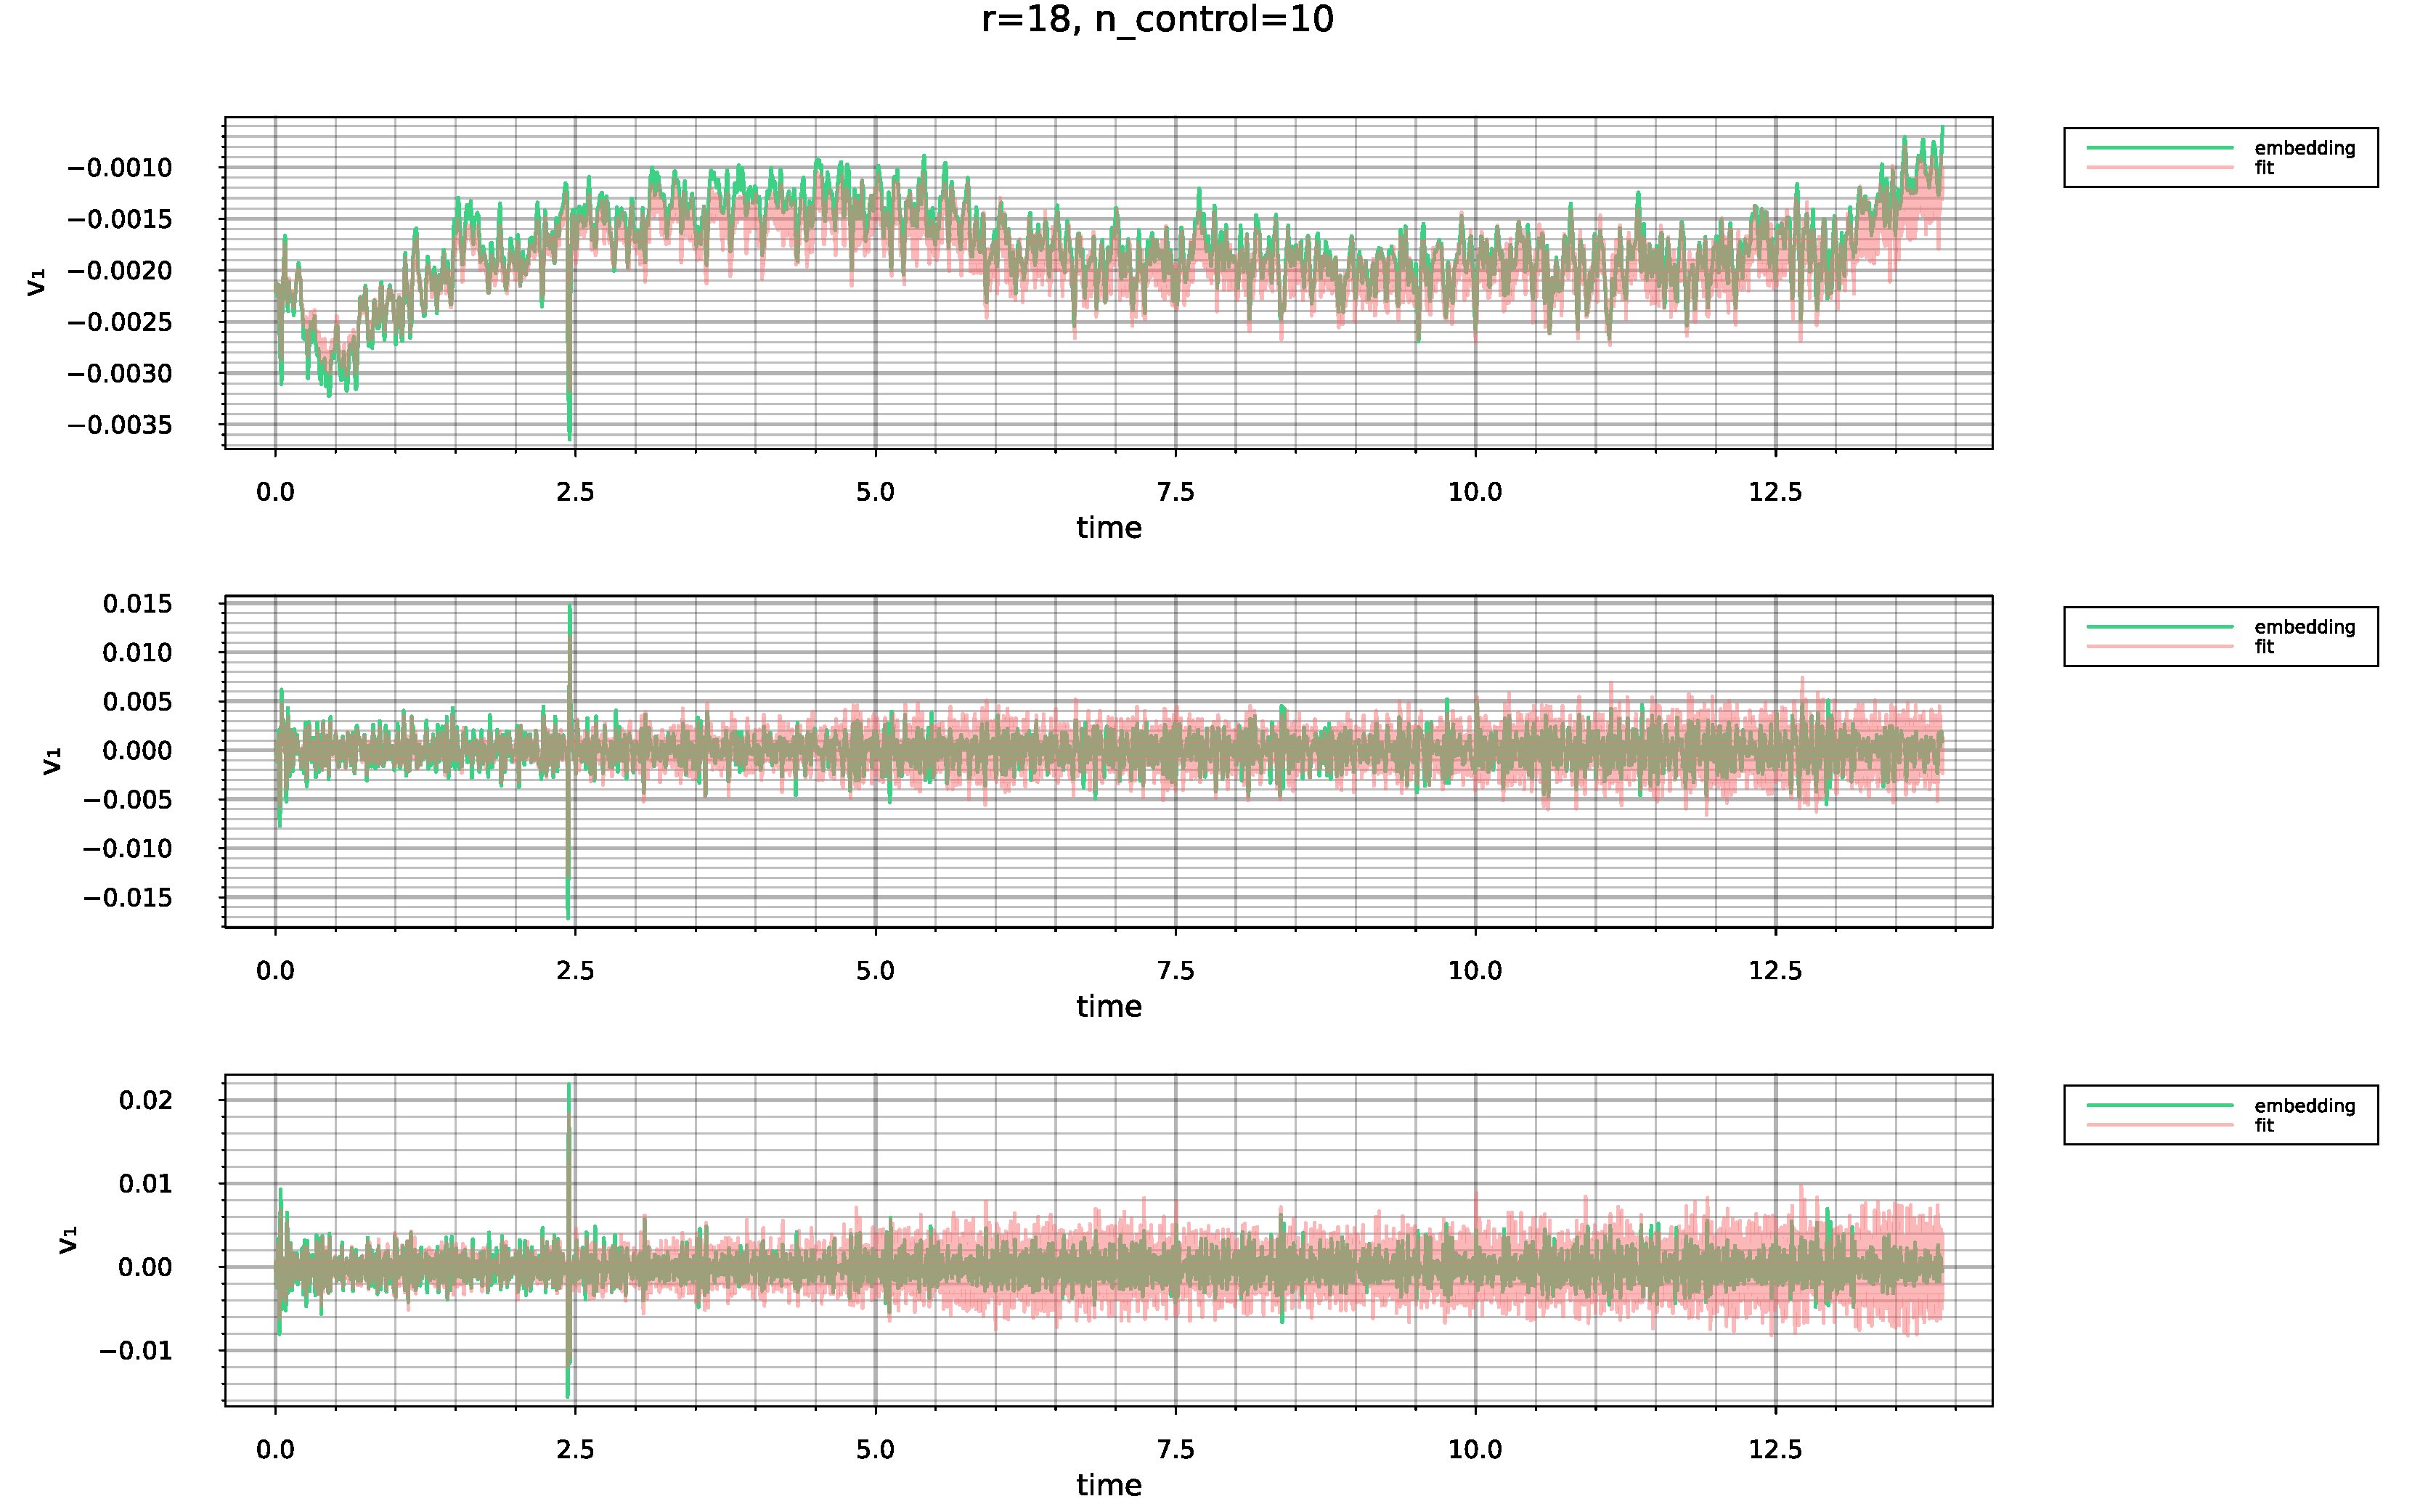
\includegraphics[width=0.85\columnwidth]{time-series/HAVOK/sharedair/havok/timeseries_reconstructed__r-18__c-10.pdf}
  \caption{The reconstructed time-series for the first three embedding coordinates using the HAVOK fit.}
  \label{fig:pm-timeseries-long}
\end{figure}
\begin{figure}[h]
  \centering
  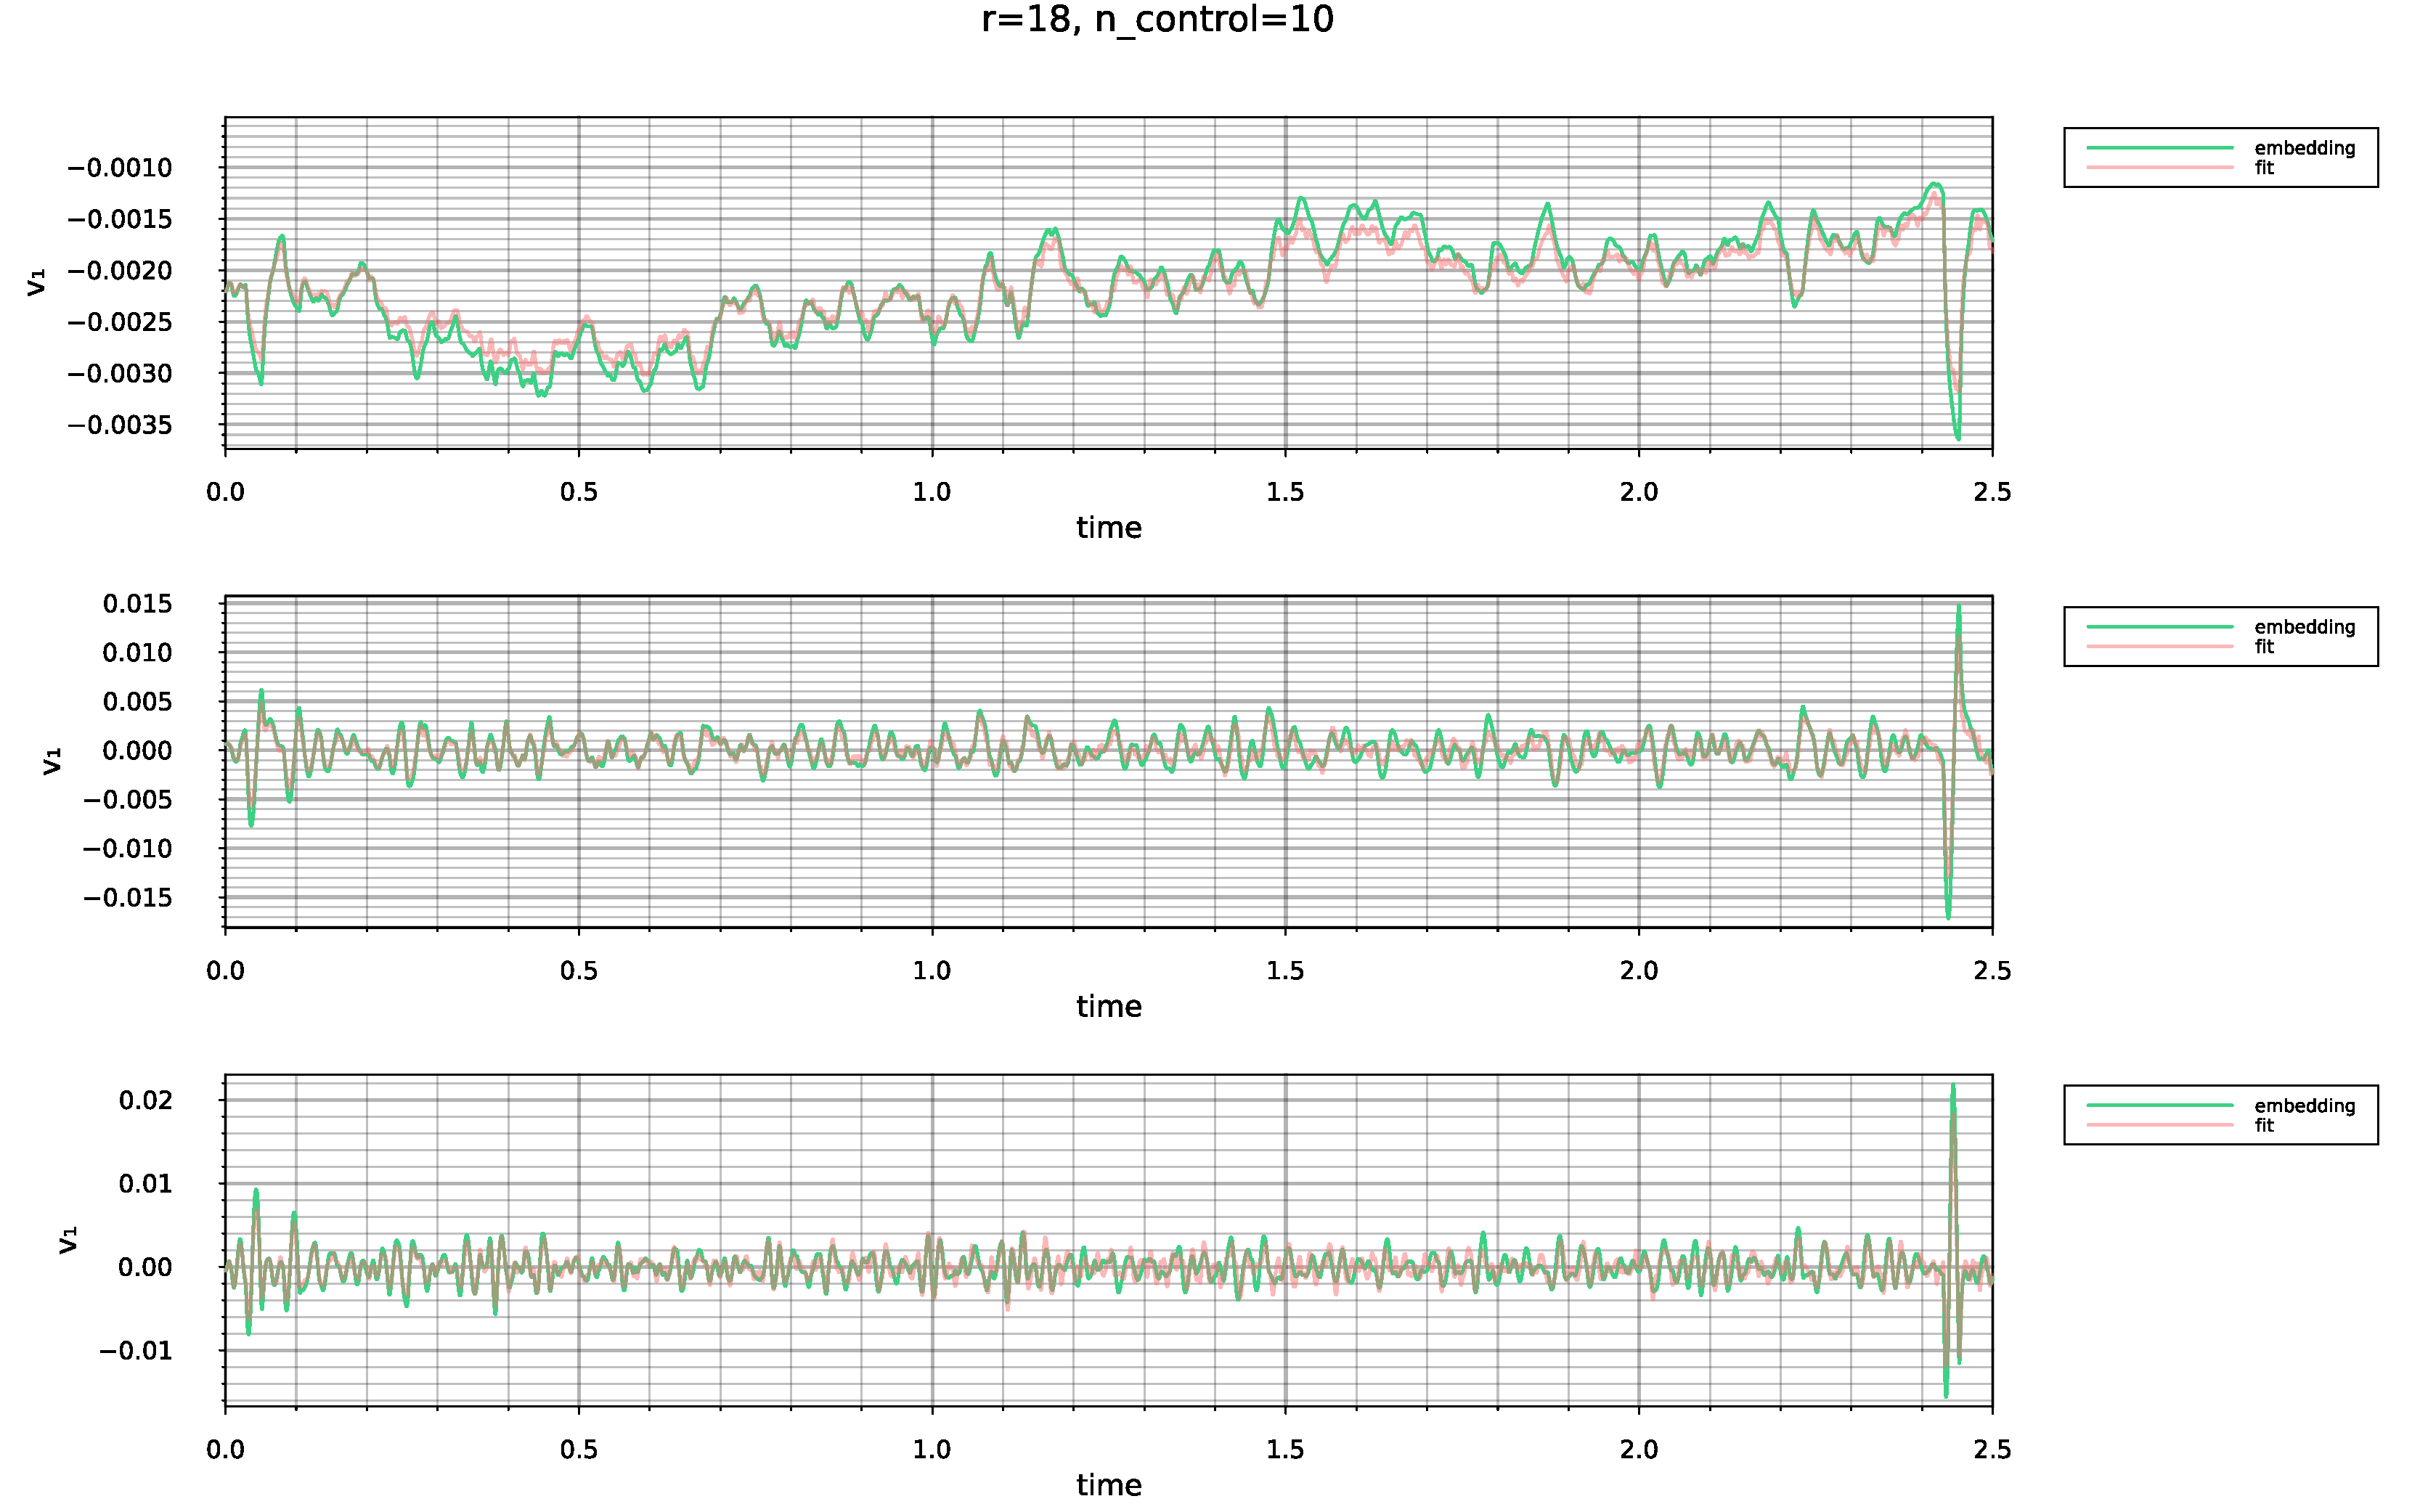
\includegraphics[width=0.85\columnwidth]{time-series/HAVOK/sharedair/havok/timeseries_reconstructed_zoomed-in.pdf}
  \caption{A zoomed in view of the same time-series reconstruction for the first $2.5$ hours showing a very decent fit. Some kind of error appears to be accumulating over time.}
  \label{fig:pm-timeseries-zoomed}
\end{figure}

Finally, if we examine the original time series and embedded attractor colored by the magnitude of the first forcing vector, we obtain Figures \ref{fig:pm-timeseries-forcing}, and \ref{fig:pm-attractor-forcing}.
\begin{figure}[h]
  \centering
  \includegraphics[width=0.85\columnwidth]{time-series/HAVOK/sharedair/havok/v1_forcing_identified.pdf}
  \caption{The first embedding coordinate with forcing above a critical threshold identified.}
  \label{fig:pm-timeseries-forcing}
\end{figure}

\begin{figure}[h]
  \centering
  \includegraphics[width=0.85\columnwidth]{time-series/HAVOK/sharedair/havok/attractor_w_forcing.png}
  \caption{The original attractor now colored by external forcing above a threshold.}
  \label{fig:pm-attractor-forcing}
\end{figure}


\subsubsection{Next Steps}

The preliminary results of our application of HAVOK to model PM data are very encouraging. The time series obtained in Figure \ref{fig:pm-timeseries-zoomed} suggest we have achieved a reasonable first order model, however as the integration period extends, the agreement is quickly lost. This is likely due to our observations not being entirely invariant under the approximated Koopman operator and therefore it is unreasonable to expect that our model will be successful with linear and external forcing terms alone. To address this, I plan to combine the HAVOK approach with the Universal Differential Equations (UDEs) framework established by Rackauckas et al in \cite{rackauckas2020universal}. That is, we can augment our learned HAVOK model to become
\begin{equation}
  \frac{d\mathbf{v}}{dt} = A\mathbf{v}(t) + Bv_{r}(t) + \text{NN}(\mathbf{v}, t)
\end{equation}
where $\text{NN}(\mathbf{v}, t)$ is a neural network. Since neural networks are universal function approximators, we can train the NN to learn the missing dynamics not present in our simple HAVOK model. Once we have accomplished this, we can then use sparse regression techniquese such as SINDy as in \cite{brunton-sindy} to obtain a functional form for the missing nonlinear terms which complete the model.


\subsection{Hamiltonian Neural Networks}

The HAVOK modeling approach outlined in the previous section can largely be understood as a \textit{data-driven} method. By carefully curating the Hankel matrix from our time series observations, we open the door to techniques from linear algebra that enable the generation of a straight-froward dynamical model. As an alternative method, let us now consider how we can use neural networks to directly model our time series data by forcing a neural network to learn useful transformations that simplify the modeling task.

For a number of years one of the most popular deep learning approaches for time series forecasting was the family of so-called \textit{recurrent neural networks} \cite{time-series-rnns}. These models take the form
\begin{equation}
  u_k = u_{k-1} + \text{NN}(u_{k-1};\theta)
\end{equation}
so that the output of the k\textsuperscript{th} layer is formed by starting with the previous output and correcting by the output of a neural network $\text{NN}(u_{k-1},\theta)$. Recently Chen et al observed that this equation can be understood to be the discrete Euler scheme implementation for a continuous ODE of the form
\begin{equation}
  \dot{u} = \text{NN}(u, \theta).
\end{equation}
Therefore, by utilizing our adjoint method for determining the sensitivity of an ODE model to the parameters $\theta$, once can construct ODE layers whose output is the solution to a differential equations \cite{neural-odes}. By extension, a reasonable time series forecasting approach would be to learn a model such that our time series $z(t)$ satisfies
\begin{equation}
  \dot{z}(t) = \text{NN}(z, t; \theta).
\end{equation}

This technique is very general however it does not take advantage of any physical constraints imposed for time series sampling real, physical processes. Much effort is now being spent on how to regularize this approach to produce physics-informed Neural ODEs such that obey physical constraints like energy conservation \cite{pinode}. Still, these physics-informed constraints are not themselves built into the model (i.e. the neural network) but rather the weights are encouraged during training to conform to physics priors. An interesting alternative development came from Greydanus et al who took a different approach by incorporating physical laws directly into the neural network structure \cite{greydanus-hnn}. Their method, the Hamiltonian Neural Network, seeks to train a neural network so that it satisfies Hamilton's equations, namely
\begin{equation}
  \begin{aligned}
    H &= \text{NN}(q,p,\theta) \\
    \dot{q} &= \frac{\partial H}{\partial p} \\
    \dot{p} &= -\frac{\partial H}{\partial q}
  \end{aligned}
\end{equation}
where $q$ and $p$ are the generalized coordinates and momenta for a system. By constructing a loss function of the form
\begin{equation}
  \mathcal{L}_{\text{HNN}} = \left\lvert \frac{\partial H}{\partial p} - \dot{q}\rvert_2 + \lvert \frac{\partial H}{\partial q} + \dot{p}\right\rvert_2
\end{equation}
they found that the HNN is able to learn a valid representation of the Hamiltonian for a variety of physical systems (spring, double pendulum, etc.). Further, since Hamilton's equations must be integrated to obtain trajectories for a system, the learned Hamiltonian can easily explore counterfactual configurations not present in the supplied training data by simply adjusting the Hamiltonian by addition of a constant (i.e. shifting the total energy). Because the total energy is a constant of motion, learning a representation of the Hamiltonian also improved the long term energy conservation of integrated trajectories as compared to directly attempting to predict $\dot{q},\dot{p}$ with a neural network alone.

To make approach feasible for real data, one must supply both position and momenta time series which may not be readily available. In their final example, the authors demonstrate how to accomplish this with an autoencoder network. By using additional encoder/decoder models, they were able to take the raw images of a \textit{video} of a swinging pendulum and \textit{learn} an effective transformation into a $q,p$ pair that they then use to learn the Haniltonian. Specifically, the HNN loss function is augmented to include two additional terms. The first is the standard autoencoder loss which demands an input that is encoded and then decoded be similar to the original input. The second is an additional loss term used to encourage the moment portion of the encoder to be some function of the velocity of the position component, that is,
\begin{equation}
  \mathcal{L}_{\text{momentum}} = \left\lvert p^t - (q^{t+1} - q^{t}) \right\rvert_2
\end{equation}



\subsubsection{Results}

I have implemented the HNN model for time series data collected by one of our central nodes. For this implementation I have joined time smoothed time series for $\text{PM}_{2.5}$ together with temperature, pressure, and humidity time series from the same node. Using this dataset with the HNN training procedure outlined above, I have been able to generate preliminary mappings of the learned Hamiltonian such as those in Figure \ref{fig:learned-hamiltonian}
\begin{figure}[h]
  \centering
  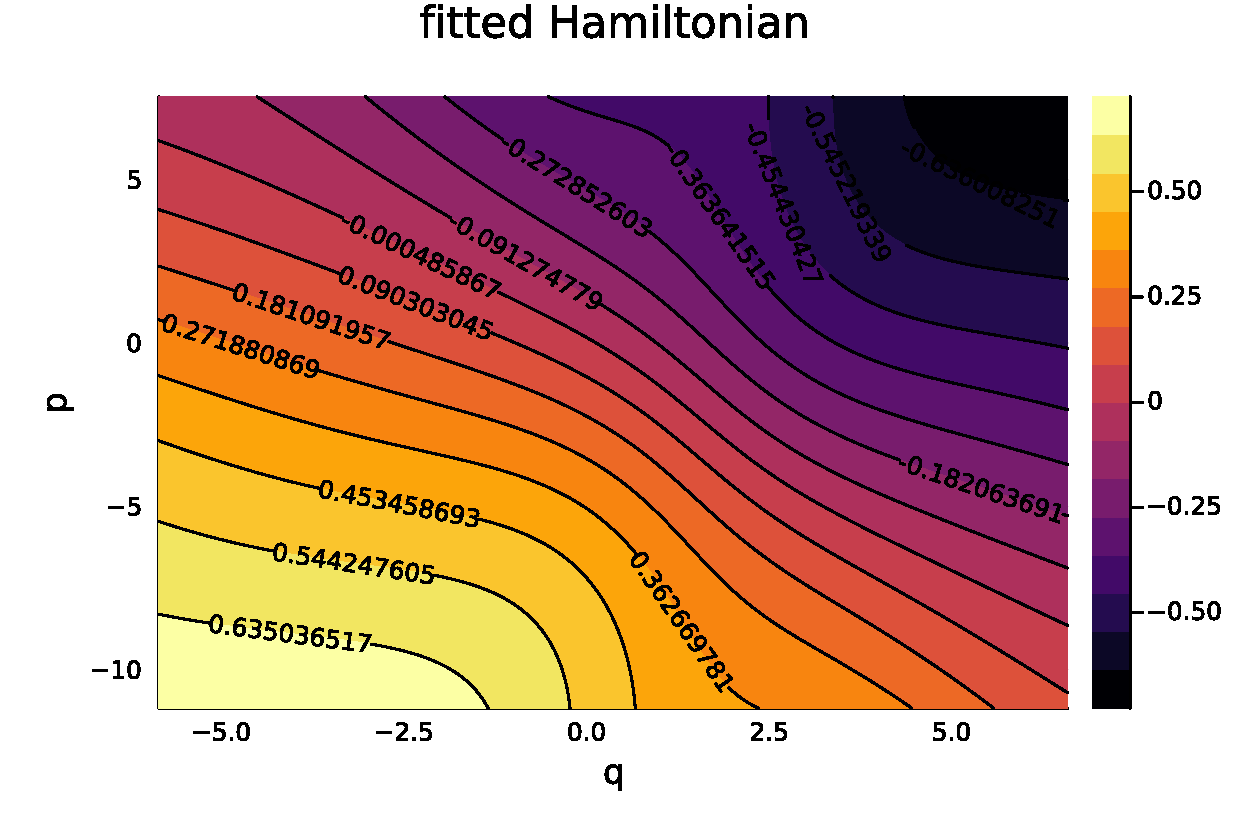
\includegraphics[width=0.85\columnwidth]{time-series/HNN/hamiltonian_cn_1--2022.pdf}
  \caption{The landscape of the Hamiltonian learned using the HNN procedure as a function of the learned phase-space coordinates $(q,p)$.}
  \label{fig:learned-hamiltonian}
\end{figure}

\subsubsection{Next Steps}

Now that I've developed the code to train an HNN, my plan is to attempt to train one for a data set consisting of roughly 1 week of observations from a Central Node to make sure we include a few iterations of the diurnal cycle. With the trained HNN we can visualize the trajectory of the system through phase space, in particular, as it relates to the level surfaces of the learned Hamiltonian. I expect that for relatively calm conditions and short time scales, the trajectories will conform to the level sets of $H$ so that the total energy is conserved. I am particularly interested in whether or not the magnitude of the gradient of $H$ can be used as an indicator of potential externel pollution sources. Similarly, I am curious about how long a trained HNN will be valid for a single sensor, as well as whether or not an HNN trained for a single node will be transferable to multiple nodes. 



%% \begin{itemize}
%% \item Uncertainty Estimation Via Time Series Sampling
%% \item Types Of Uncertainty
%% \item Instrument Uncertainty
%% \item Representativeness Uncertainty
%% \item Variograms
%% \item Mutual Information
%% \item Auto-correlation
%% \item Time Series Chaos
%% \item What is Chaos?
%% \item Lyapunov Exponents
%% \item Fractal Dimension
%% \item Koopman Operator Theory
%% \item Time Series Modeling Methods
%% \item Token-Hankel Delay Embeddings
%% \item Embedding Theorems (are magic)
%% \item Determination of Optimal Lag
%% \item Determination of Intrinsic Dimension (kind of unnecessary given *large enough* embedding)
%% \item DMD and HAVOK
%% \item Hamiltonian Neural Networks
%% \item Time Series Classification
%% \item Considerations for Batching of Time Series for ML Models
%% \item K-means Clustering
%% \item Self Organizing Maps
%% \item Generative Topographic Maps
%% \item Chaos Classification via HAVOK
%% \item Symplectic and Normal Gradients for HNN
%% \item Motivating Example: Lorenz63 System
%% \item Origin of Lorenz System
%% \item Time Scale Analysis and Variography
%% \item Embedding
%% \item Modeling
%% \item Classification
%% \item Real Example 1: PM Data
%% \item Origin of Lorenz System
%% \item Time Scale Analysis and Variography
%% \item Embedding
%% \item Modeling
%% \item Classification
%% \item Real Example 2: Biometric Data
%% \item Origin of Lorenz System
%% \item Time Scale Analysis and Variography
%% \item Embedding
%% \item Modeling
%% \item Classification
%% \item Real Example 3: Stock Market Analysis
%% \item Origin of Lorenz System
%% \item Time Scale Analysis and Variography
%% \item Embedding
%% \item Modeling
%% \item Classification
%% \end{itemize}
